\documentclass{article}
\usepackage{tikz}
\usetikzlibrary{shapes.geometric}

\begin{document}

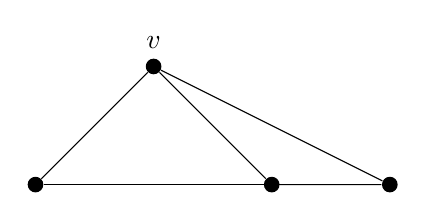
\begin{tikzpicture}[scale=1.5]
    % Define nodes
    \node (v) at (0,0) [circle,fill,inner sep=2pt] {};
    \node (a) at (-1,-1) [circle,fill,inner sep=2pt] {};
    \node (b) at (1,-1) [circle,fill,inner sep=2pt] {};
    \node (c) at (2,-1) [circle,fill,inner sep=2pt] {};

    % Draw edges
    \draw (v) -- (a);
    \draw (v) -- (b);
    \draw (v) -- (c);
    \draw (a) -- (b);
    \draw (b) -- (c);
    \draw (c) -- (a);

    % Label node v
    \node at (0,0.2) {$v$};
\end{tikzpicture}

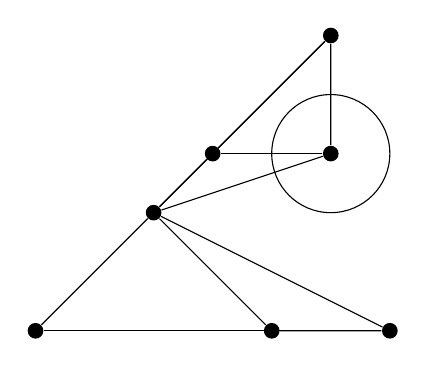
\begin{tikzpicture}[scale=1.5]
    % Define nodes
    \node (v) at (0,0) [circle,fill,inner sep=2pt] {};
    \node (a) at (-1,-1) [circle,fill,inner sep=2pt] {};
    \node (b) at (1,-1) [circle,fill,inner sep=2pt] {};
    \node (c) at (2,-1) [circle,fill,inner sep=2pt] {};
    \node (d) at (0.5,0.5) [circle,fill,inner sep=2pt] {};
    \node (e) at (1.5,0.5) [circle,fill,inner sep=2pt] {};
    \node (f) at (1.5,1.5) [circle,fill,inner sep=2pt] {};

    % Draw edges
    \draw (v) -- (a);
    \draw (v) -- (b);
    \draw (v) -- (c);
    \draw (a) -- (b);
    \draw (b) -- (c);
    \draw (c) -- (a);
    \draw (d) -- (e);
    \draw (e) -- (f);
    \draw (f) -- (d);
    \draw (v) -- (d);
    \draw (v) -- (e);
    \draw (v) -- (f);

    % Draw circle
    \draw (1.5,0.5) circle (0.5);
\end{tikzpicture}

\end{document}